% version 1.00, date 11/11/16, auteur Kafui Atanley

Ce chapitre décrit les différents cas d'utilisation pour chaque fonctionnalité.

\section{Lot 2}
\subsection{Fonctionnalité 1}
Ce paragraphe décrit les cas d'utilisation concernant la fonctionnalité 1. \\

La figure suivante (figure \ref{diagrammeCasUtilisation1-1}) indique les cas d'utilisation pour la gestion de comptes lorsque l'utilisateur est connecté.
\begin{figure}[H]
	\centering
	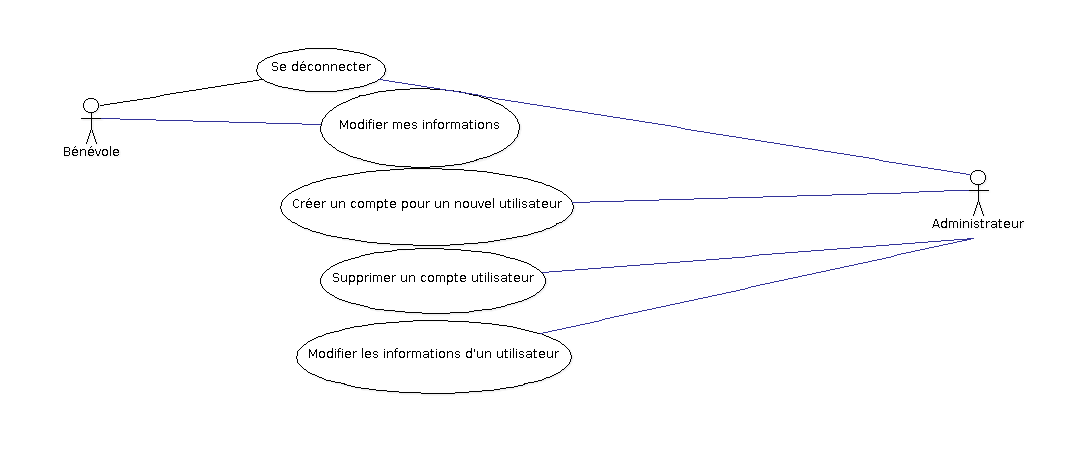
\includegraphics[scale=0.40]{casDUtilisation/images/fonctionnalite1UtilisateurConnecte.png}
	\caption{Cas d'utilisation~: Gestion de compte utilisateur connecté }
	\label{diagrammeCasUtilisation1-1}
\end{figure}

La figure suivante (figure \ref{diagrammeCasUtilisation1-2}) indique les cas d'utilisation pour la gestion de comptes lorsque l'utilisateur est déconnecté.
\begin{figure}[H]
	\centering
	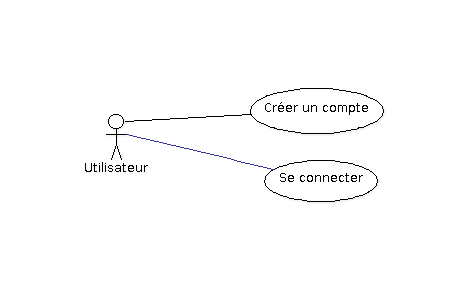
\includegraphics[scale=0.60]{casDUtilisation/images/fonctionnalite1UtilisateurNonConnecte.png}
	\caption{Cas d'utilisation~: Gestion de compte utilisateur déconnecté}
	\label{diagrammeCasUtilisation1-2}
\end{figure}

\subsection{Fonctionnalité 2}
Ce paragraphe décrit le cas d'utilisation concernant la fonctionnalité 2. \\

La figure suivante (figure \ref{diagrammeCasUtilisation2}) indique les cas d'utilisation pour de la création, la modification et la suppression d'un établissement par un administrateur.
\begin{figure}[H]
	\centering
	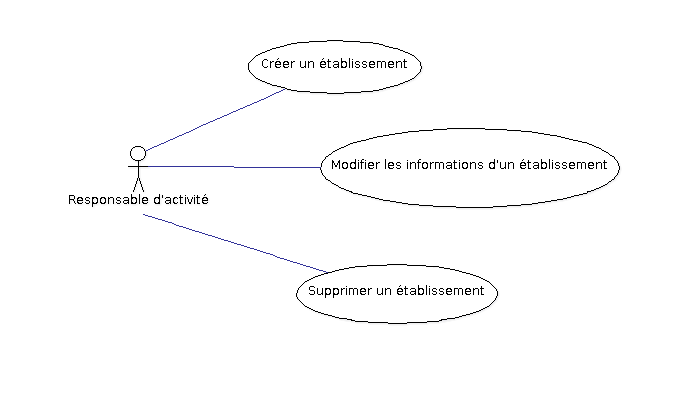
\includegraphics[scale=0.5]{casDUtilisation/images/fonctionnalite2Etablissement.png}
	\caption{Cas d'utilisation~: Création, modification, suppression d'un établissement par un administrateur}
	\label{diagrammeCasUtilisation2}
\end{figure}

\subsection{Fonctionnalité 3}
Ce paragraphe décrit le cas d'utilisation concernant la fonctionnalité 3. \\

La figure suivante (figure \ref{diagrammeCasUtilisation3}) indique les cas d'utilisation pour l'envoi du formulaire de demande d'intervention aux établissements.
\begin{figure}[H]
	\centering
	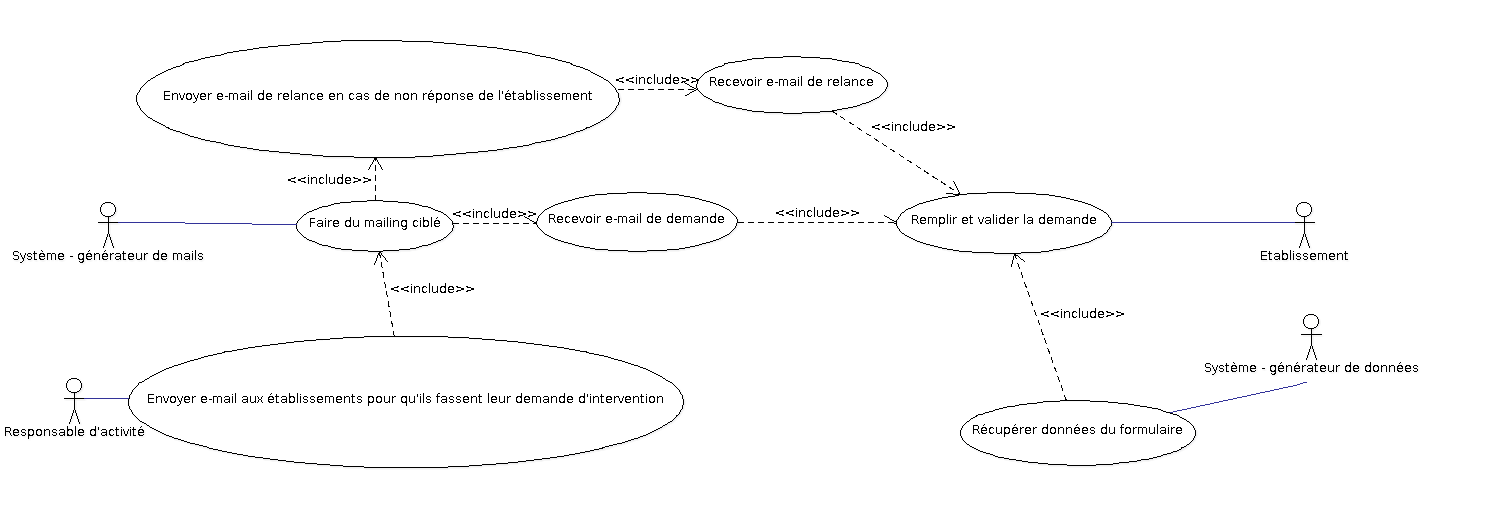
\includegraphics[scale=0.3]{casDUtilisation/images/fonctionnalite3Mailing.png}
	\caption{Cas d'utilisation~: Envoi du formulaire à un ensemble d'établissement}
	\label{diagrammeCasUtilisation3}
\end{figure}

\subsection{Fonctionnalité 4}
Ce paragraphe décrit les cas d'utilisation concernant la fonctionnalité 4. \\

La figure suivante (figure \ref{diagrammeCasUtilisation4}) indique les cas d'utilisation pour le remplissage du formulaire de demande d'intervention.
\begin{figure}[H]
	\centering
	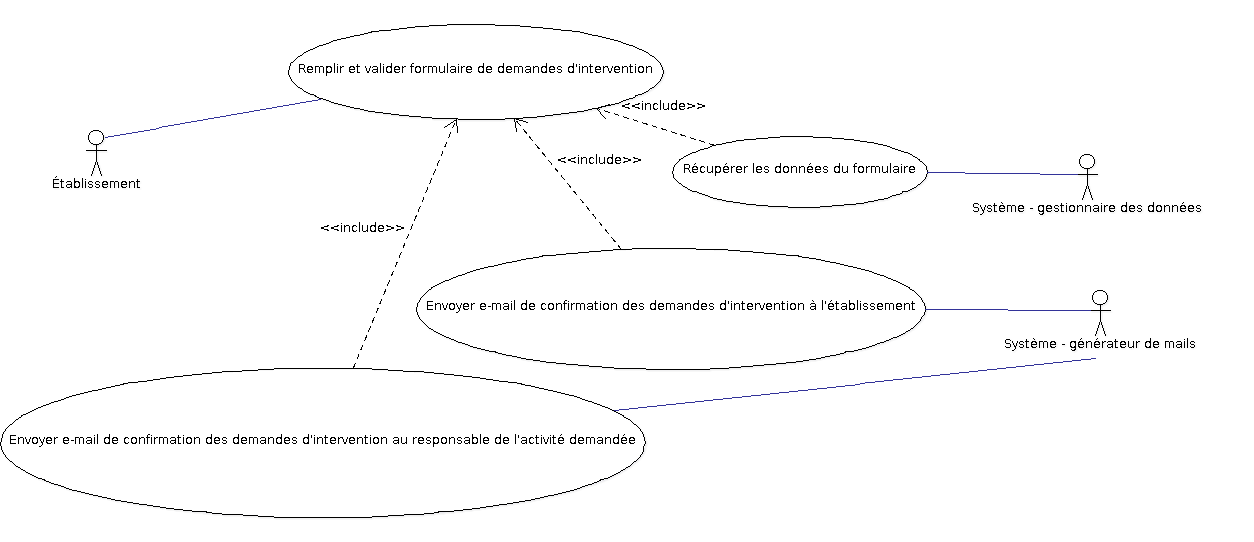
\includegraphics[scale=0.4]{casDUtilisation/images/fonctionnalite4ReceptionIntervention.png}
	\caption{Cas d'utilisation~: Replissage du formulaire}
	\label{diagrammeCasUtilisation4}
\end{figure}

\subsection{Fonctionnalité 5}
Ce paragraphe décrit le cas d'utilisation concernant la fonctionnalité 5. \\

La figure suivante (figure \ref{diagrammeCasUtilisation5}) indique les cas d'utilisation pour la géolocalisation des interventions ainsi que l'affectation d'un plaideur à celles ci. \\
\begin{figure}[H]
	\centering
	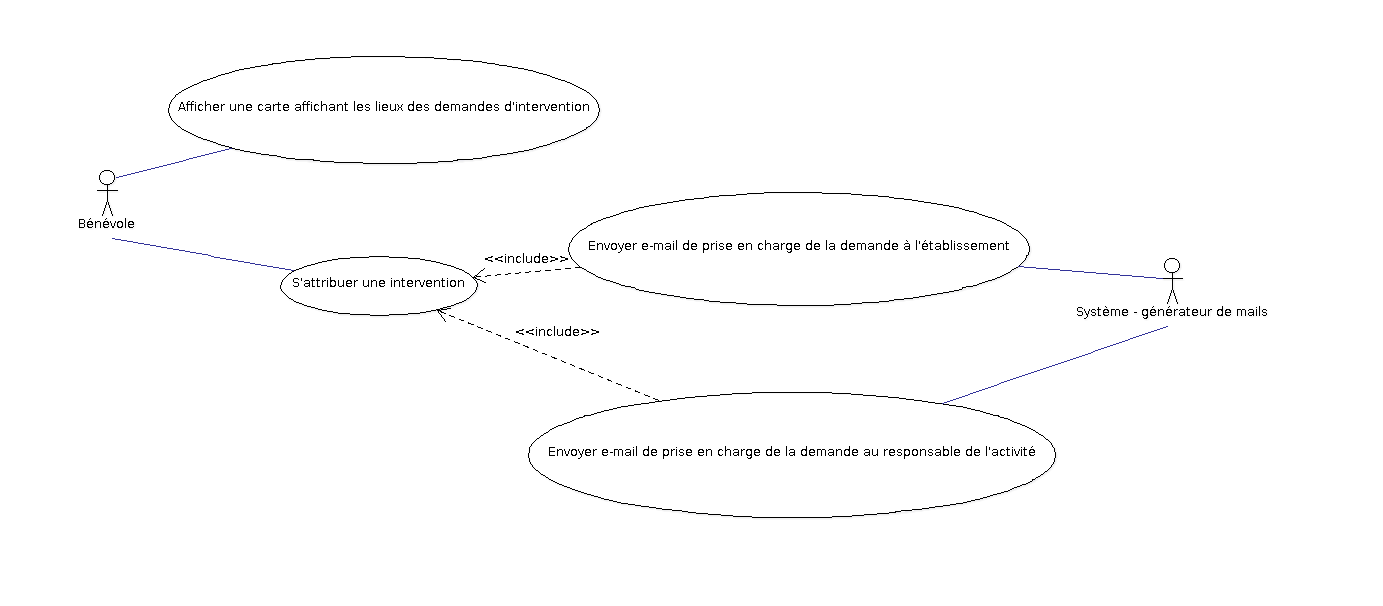
\includegraphics[scale=0.35]{casDUtilisation/images/fonctionnalite5Attribution.png}
	\caption{Cas d'utilisation~: Géolocalisation des interventions et affectation à une intervention}
	\label{diagrammeCasUtilisation5}
\end{figure}

\subsection{Fonctionnalité 6}
Ce paragraphe décrit le cas d'utilisation concernant la fonctionnalité 6. \\

La figure suivante (figure \ref{diagrammeCasUtilisation6}) indique les cas d'utilisation de la mise à jour du planning d'un plaideur et l'information de prise en charge de l'intervention à l'établissement.
\begin{figure}[H]
	\centering
	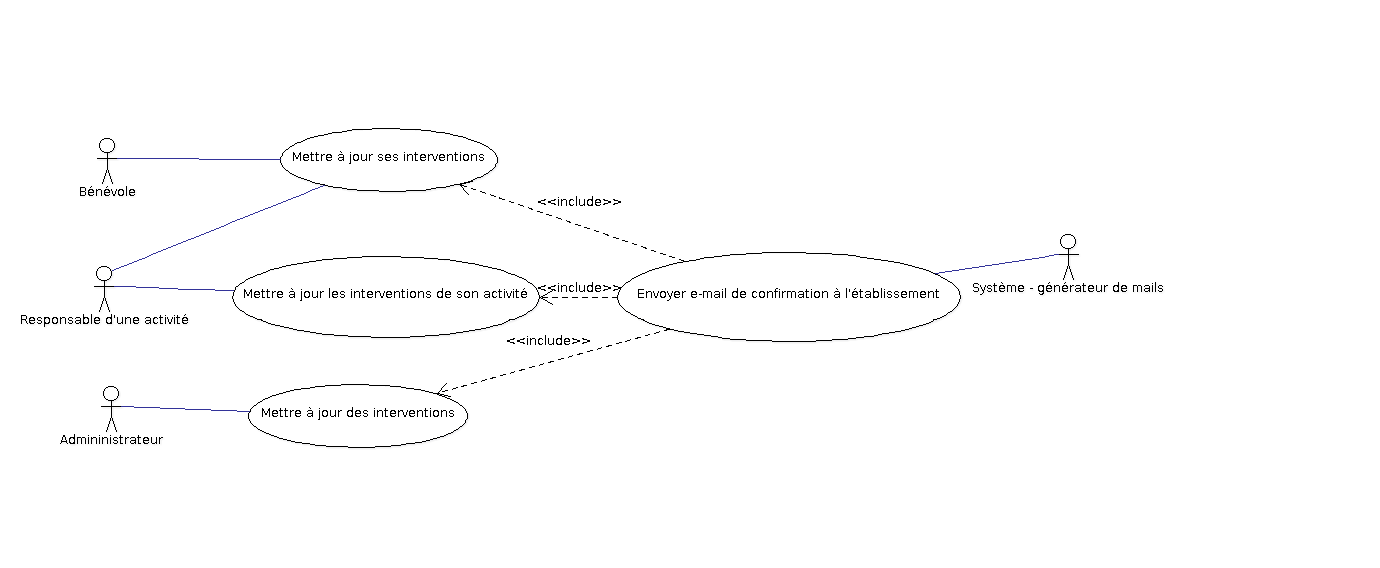
\includegraphics[scale=0.4]{casDUtilisation/images/fonctionnalite6MiseAJourIntervention.png}
	\caption{Cas d'utilisation~: Mise à jour du planning d'un plaideur et information à l'établissement}
	\label{diagrammeCasUtilisation6}
\end{figure}

\subsection{Fonctionnalité 7}
Ce paragraphe décrit le cas d'utilisation concernant la fonctionnalité 7.\\

La figure suivante (figure \ref{diagrammeCasUtilisation7}) indique les cas d'utilisation pour l'envoi des emails de rappel au plaideur et à l'établissement.
\begin{figure}[H]
	\centering
	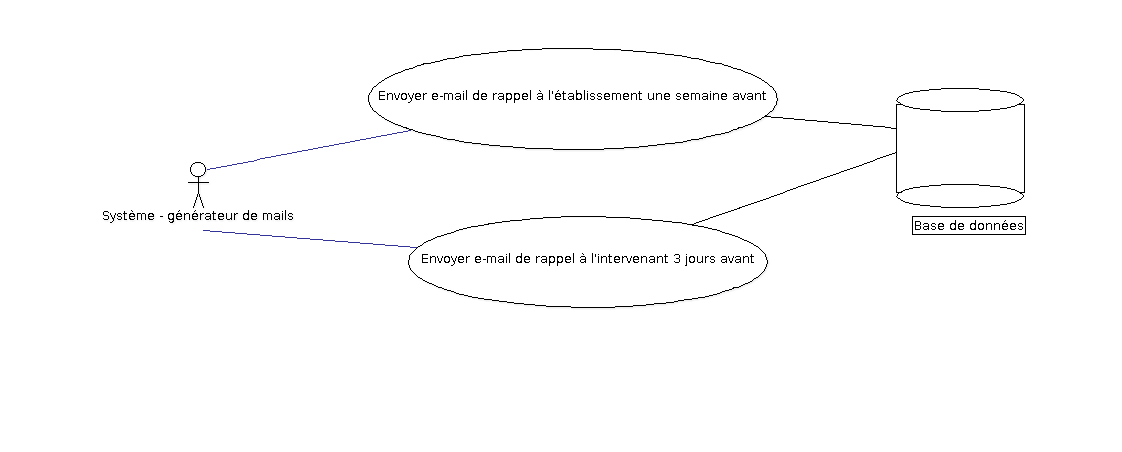
\includegraphics[scale=0.4]{casDUtilisation/images/fonctionnalite7Rappels.png}
	\caption{Cas d'utilisation~: Envoi des emails de rappel}
	\label{diagrammeCasUtilisation7}
\end{figure}

\section{Lot 3}
\subsection{Fonctionnalité 8}
Ce paragraphe décrit les cas d'utilisation concernant la fonctionnalité 8 soit la géolocalisation. \\

La figure suivante (figure \ref{diagrammeCasUtilisation8}) indique les cas d'utilisation pour la géolocalisation.
\begin{figure}[H]
	\centering
	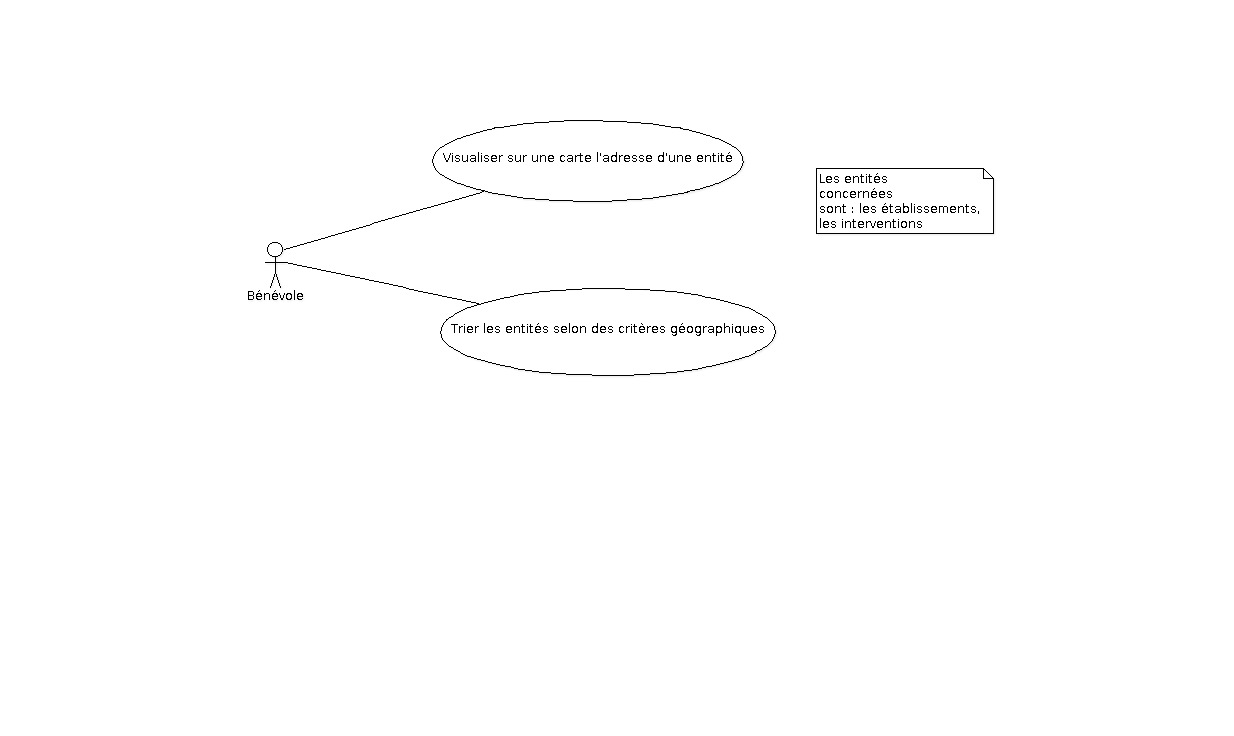
\includegraphics[scale=0.40]{casDUtilisation/images/fonctionnalite8Geolocalisation.png}
	\caption{Cas d'utilisation~: Géolocalisation }
	\label{diagrammeCasUtilisation8}
\end{figure}

\subsection{Fonctionnalité 9}
Ce paragraphe décrit les cas d'utilisation concernant la fonctionnalité 9 soit l'attribution de frimousse. \\

La figure suivante (figure \ref{diagrammeCasUtilisation9}) indique les cas d'utilisation pour l'attribution de frimousse.
\begin{figure}[H]
	\centering
	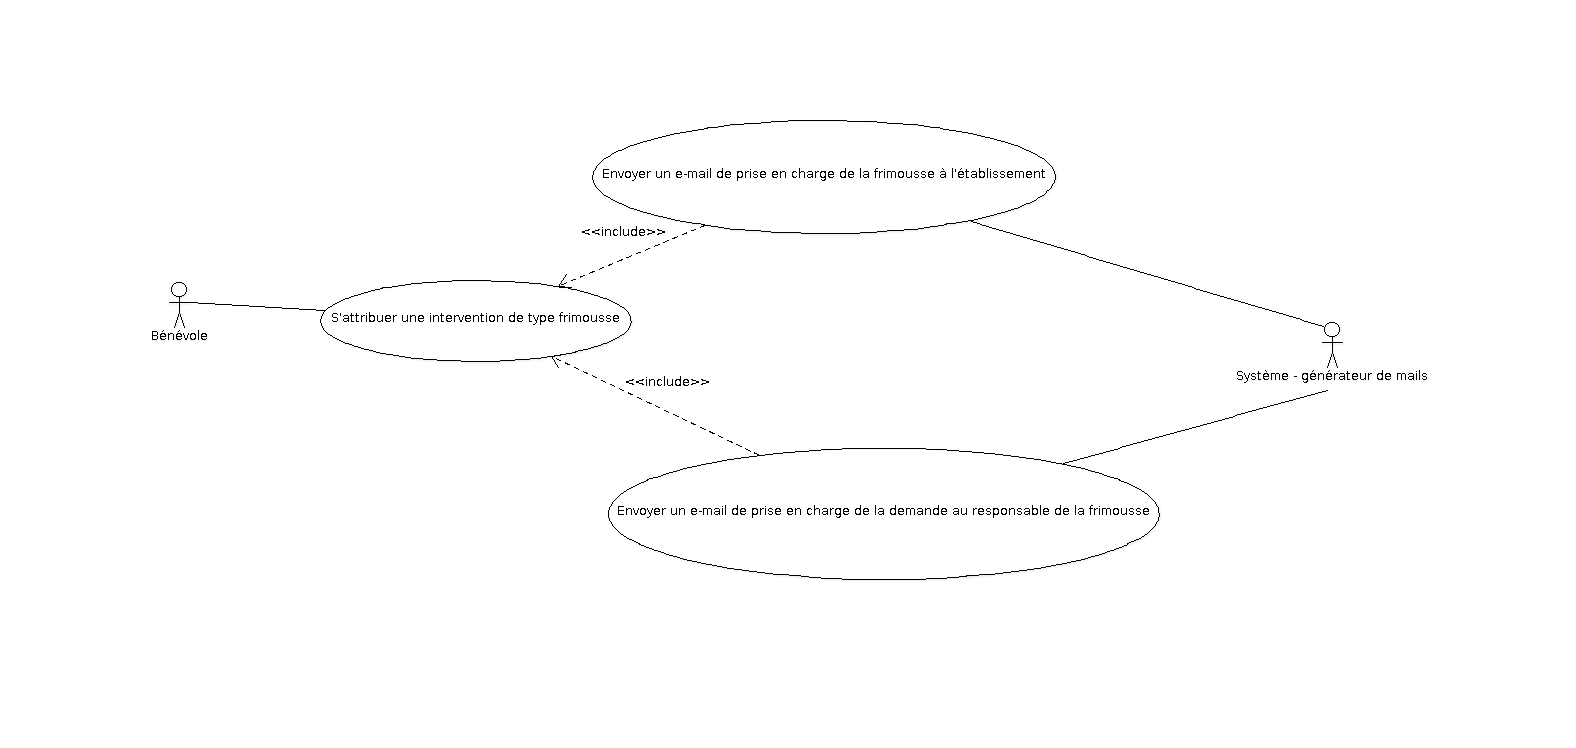
\includegraphics[scale=0.35]{casDUtilisation/images/fonctionnalite9Attribution.png}
	\caption{Cas d'utilisation~: Attribution de frimousse }
	\label{diagrammeCasUtilisation9}
\end{figure}

\subsection{Fonctionnalité 10}
Ce paragraphe décrit les cas d'utilisation concernant la fonctionnalité 10 soit la gestion des ventes. \\

La figure suivante (figure \ref{diagrammeCasUtilisation10}) indique les cas d'utilisation pour l'attribution de frimousse.
\begin{figure}[H]
	\centering
	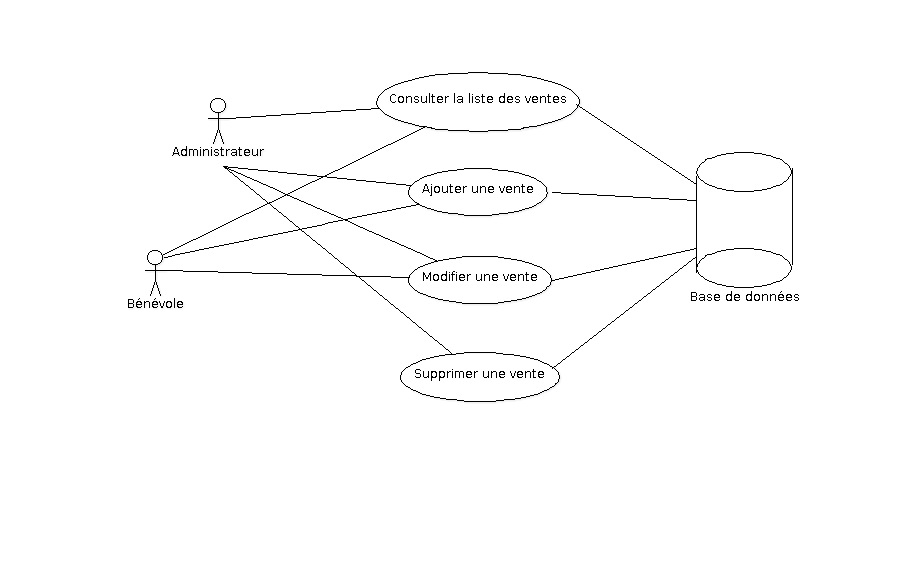
\includegraphics[scale=0.40]{casDUtilisation/images/fonctionnalite10Vente.png}
	\caption{Cas d'utilisation~: Gestion des ventes }
	\label{diagrammeCasUtilisation10}
\end{figure}
